\begin{figure}
\centering
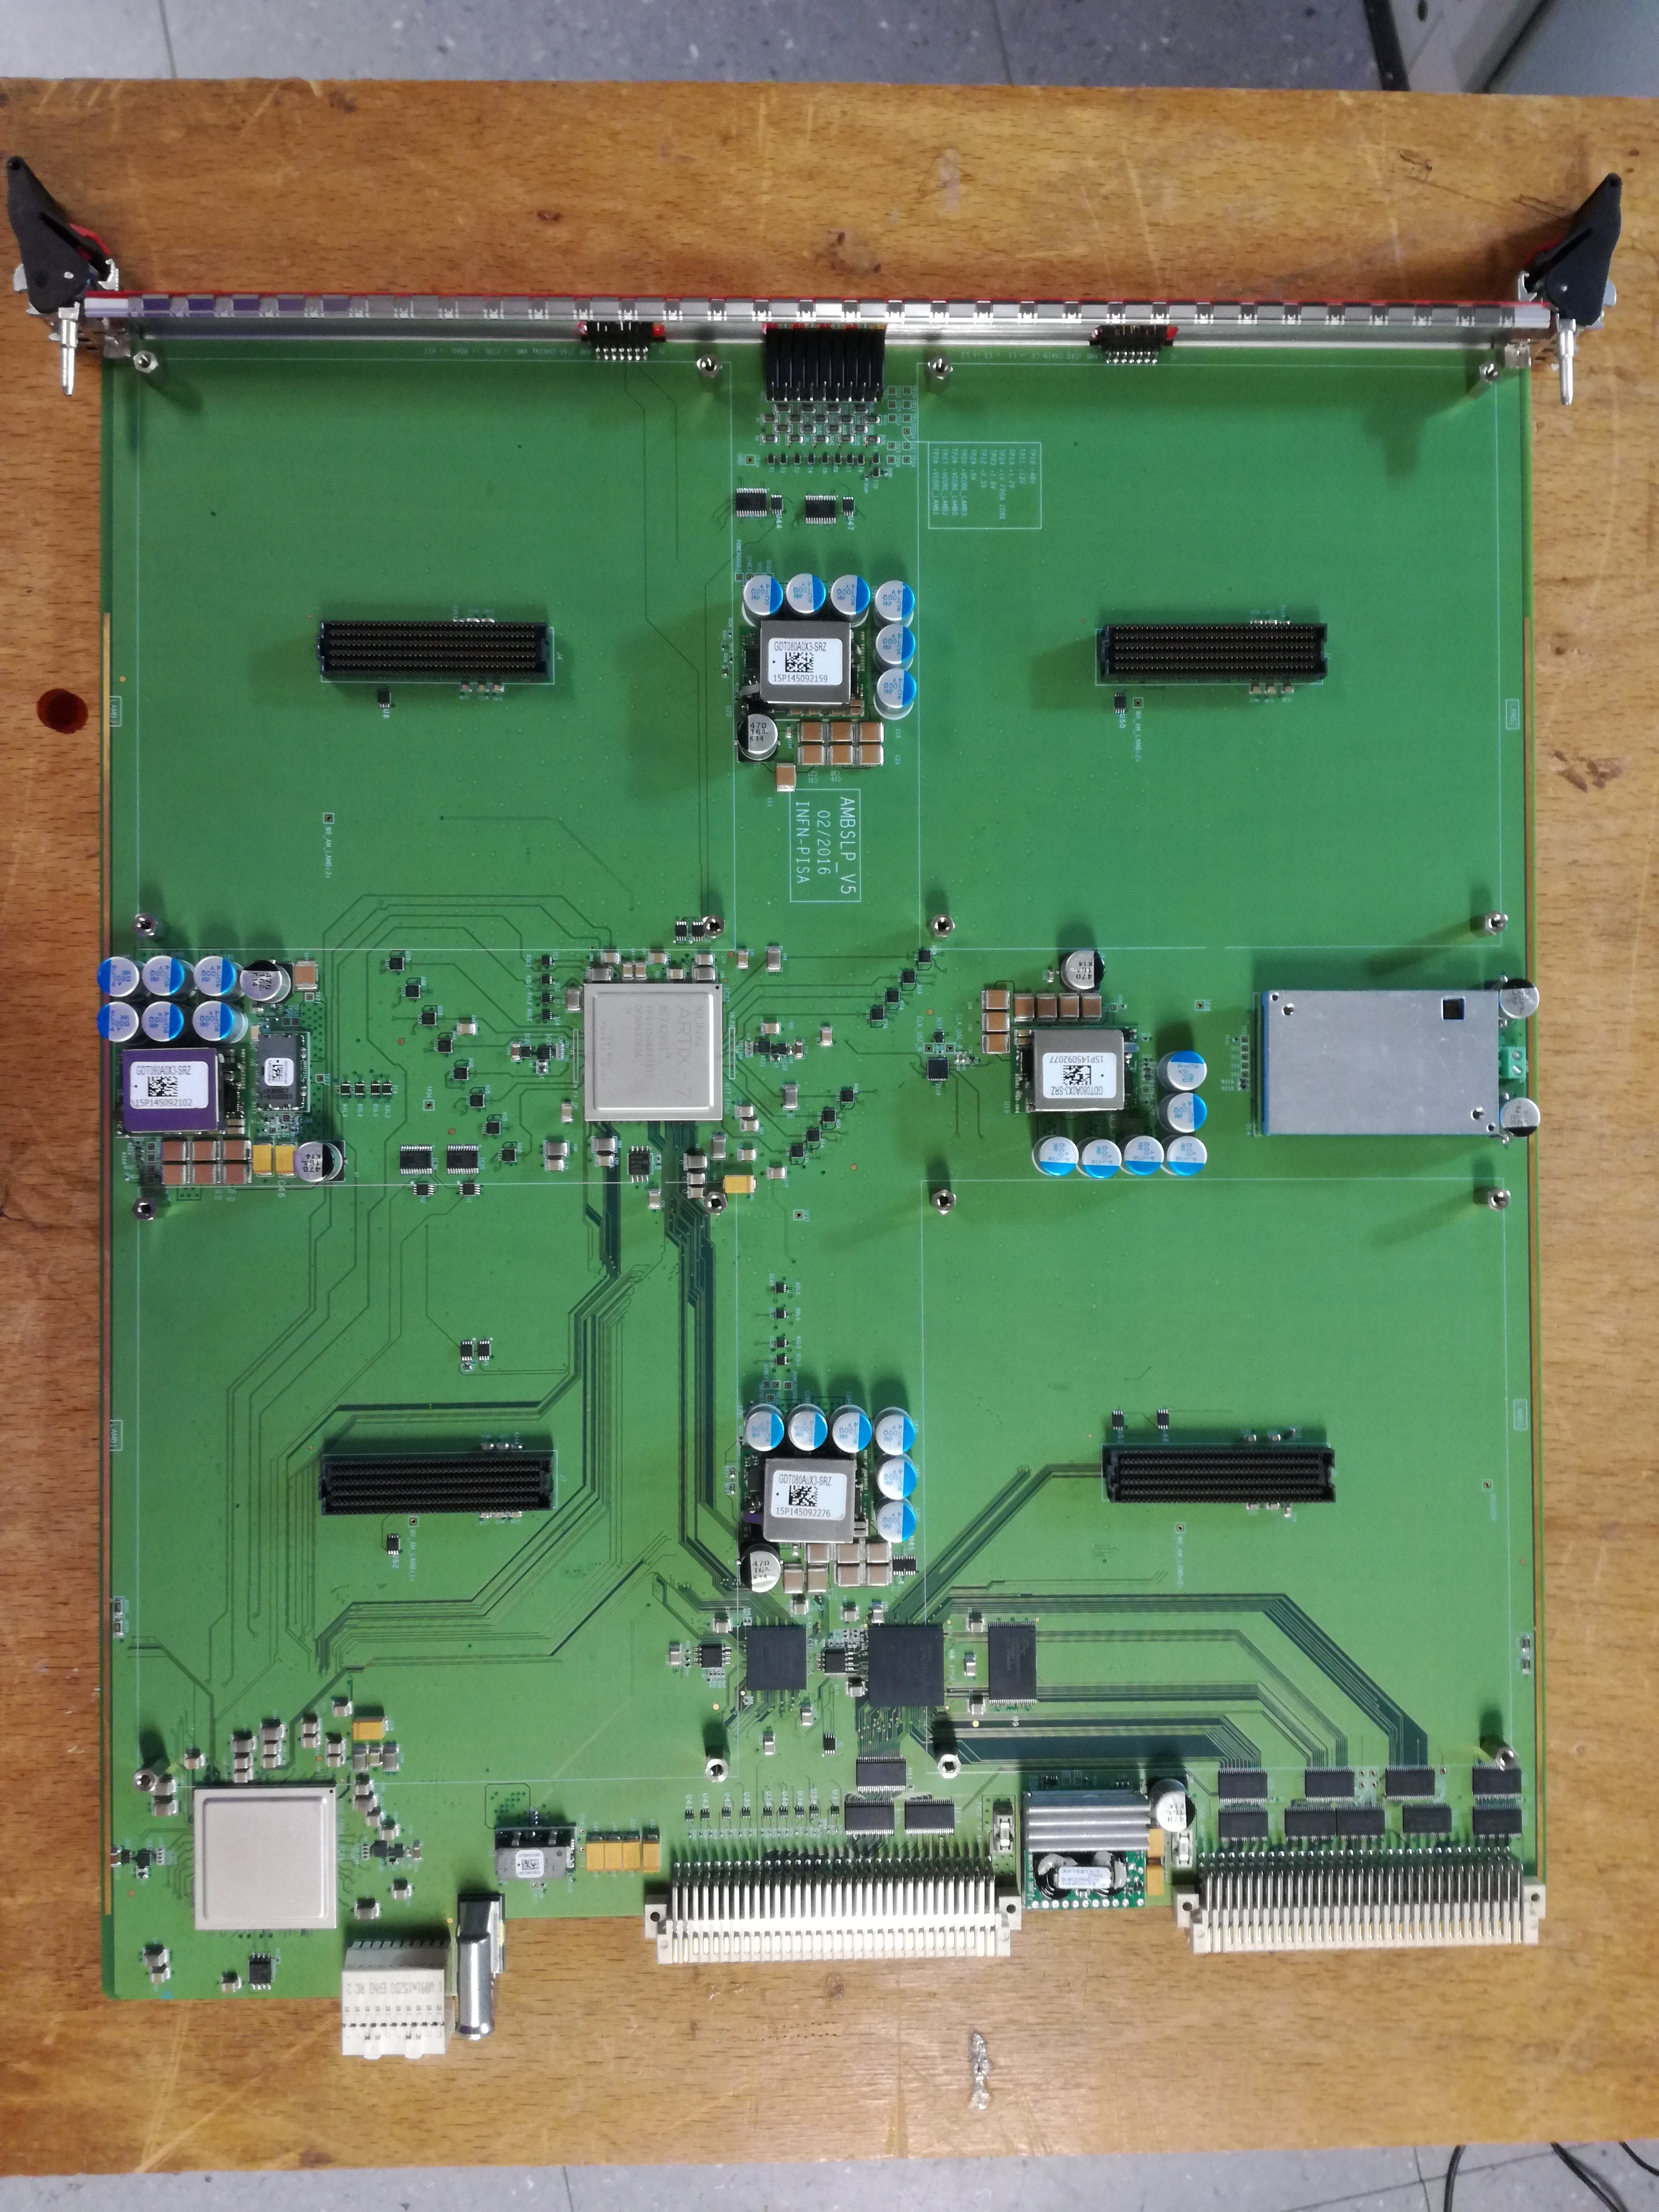
\includegraphics[width=.6\linewidth,angle=90]{Images/AMBoard.jpg}
\caption{The picture shows an AMBoard, top side. The 4 FPGAs are
clearly visible. The four FMC connectors show where the LAMBs wil be
installed}
\label{fig:amboard_top}
\end{figure}

\begin{figure}
\centering

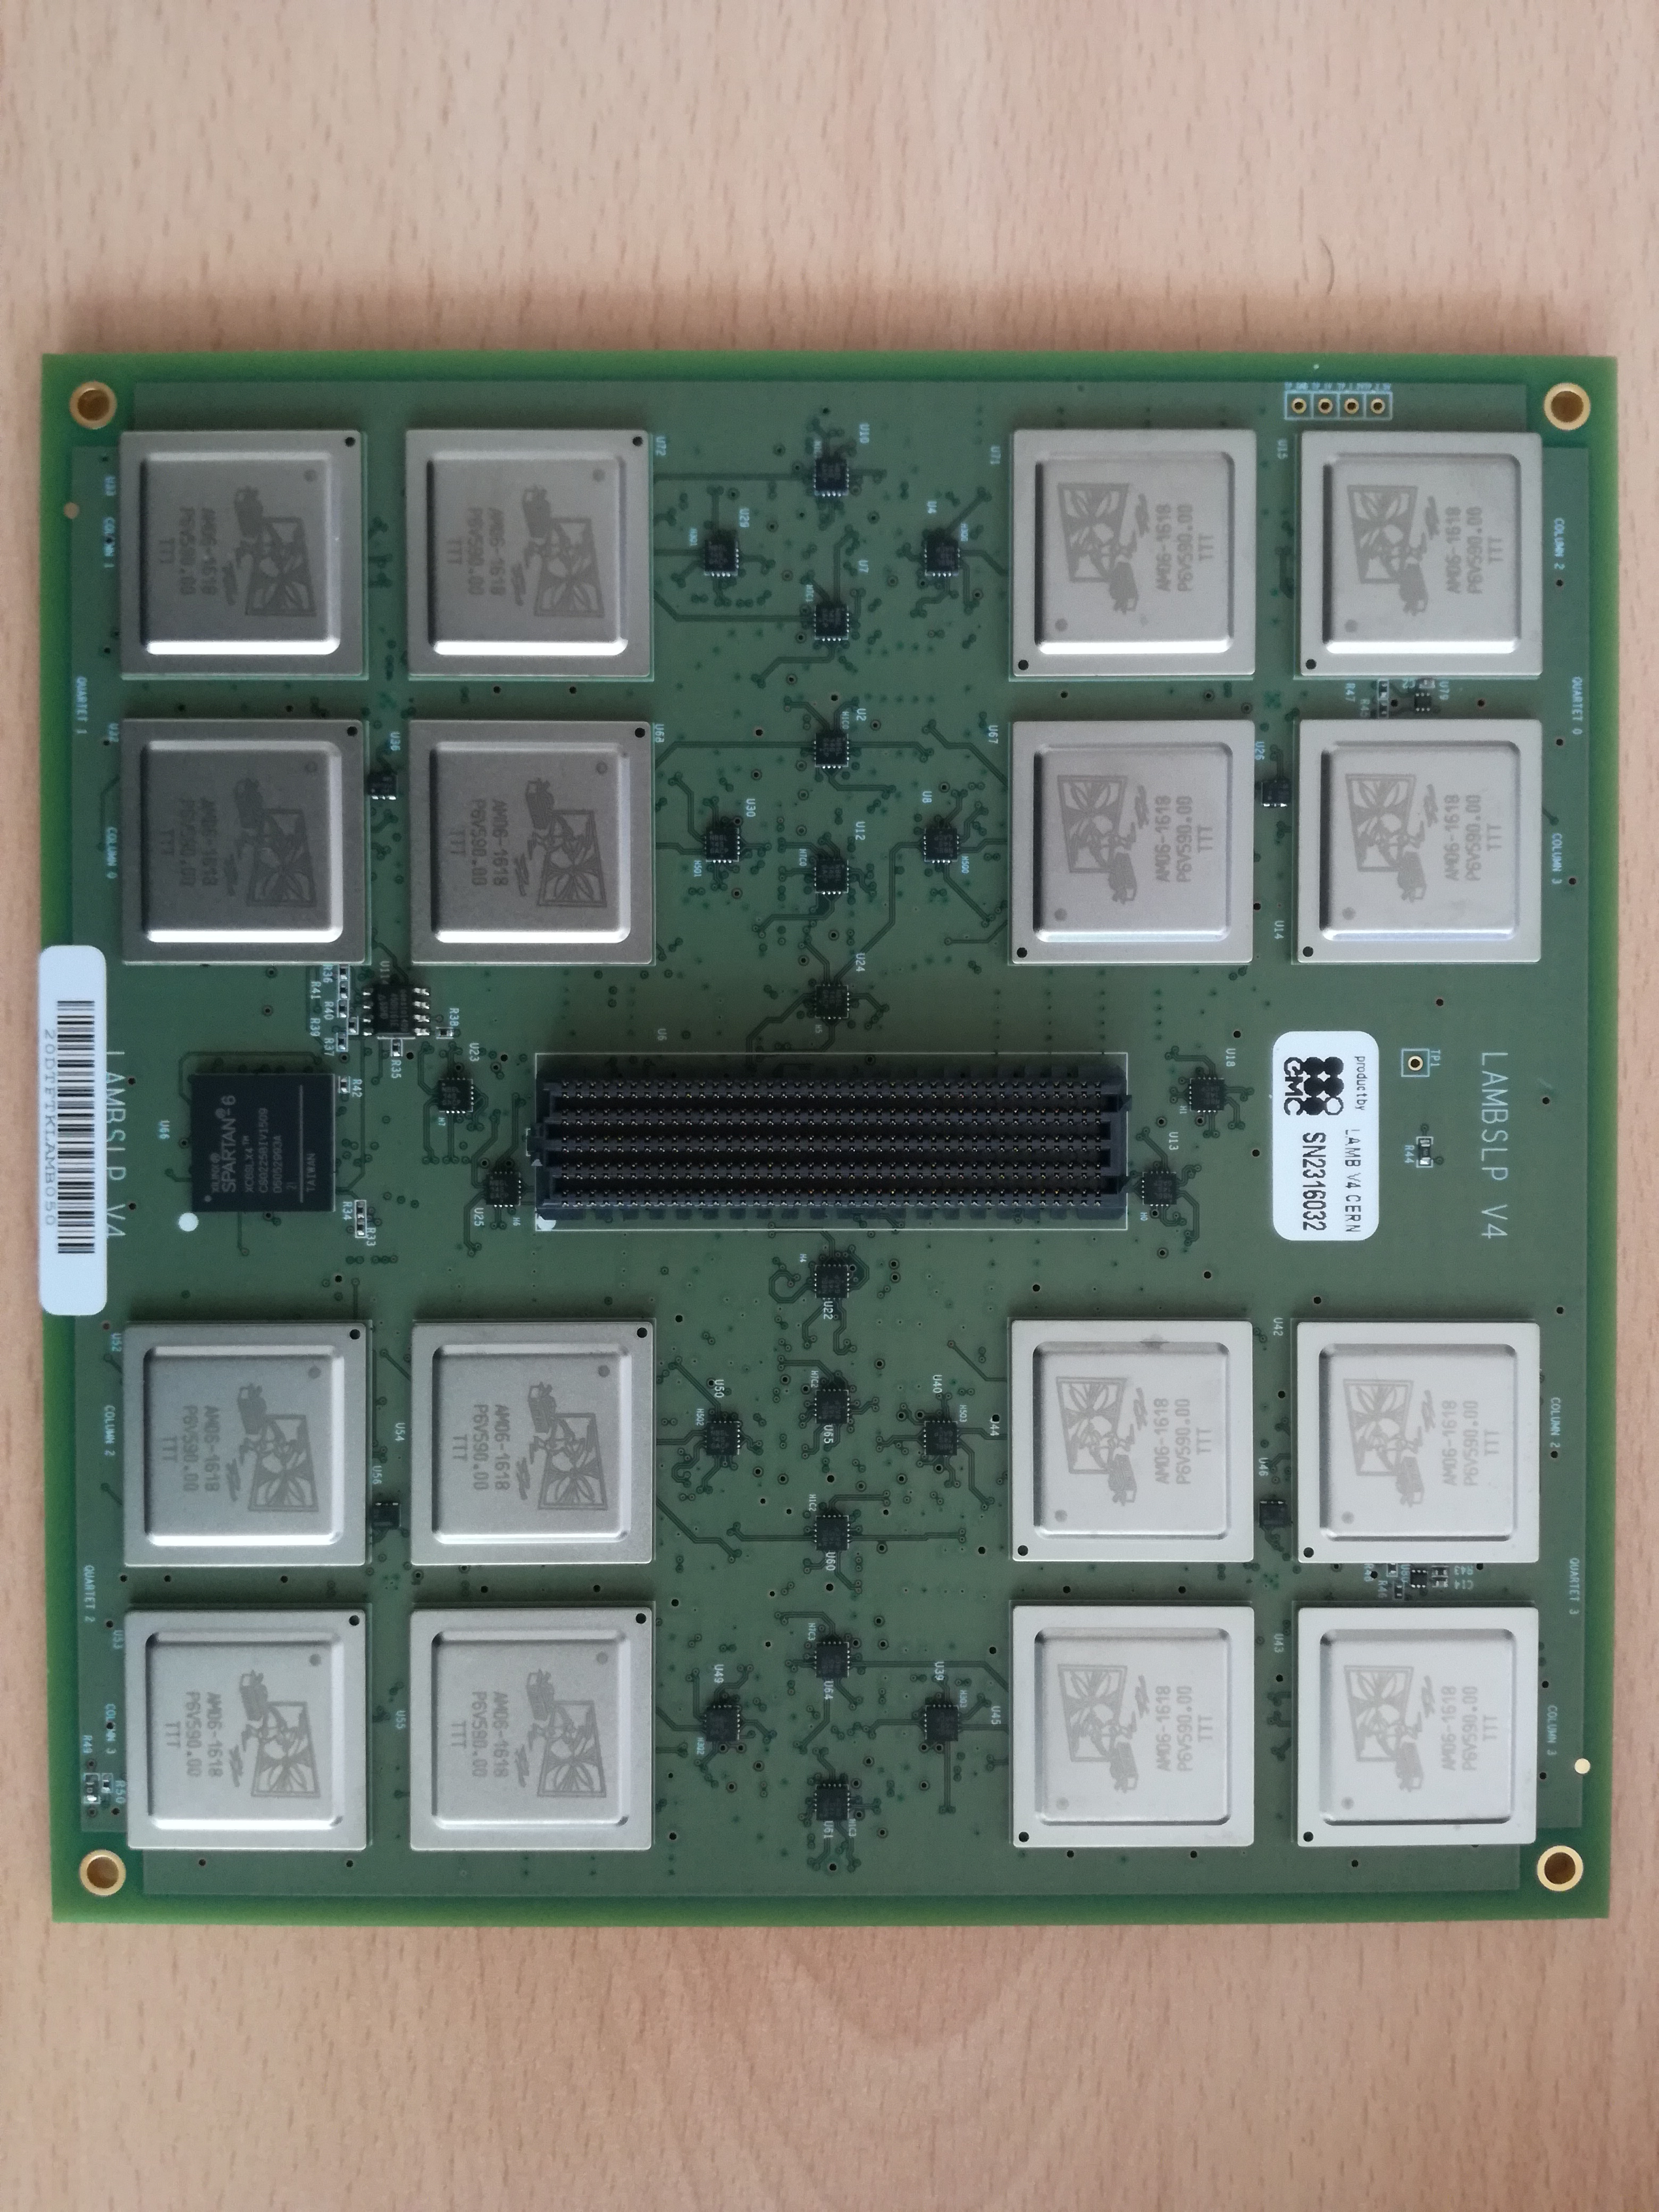
\includegraphics[width=.4\linewidth,angle=90]{Images/LAMB.jpg}

\caption{The figure shows a LAMB mezzanine, from the side that faces
the AMB and where the chips are installed. The organization of the chips
as quartets and the fan-out chips are clearly visible. The BUSCA
chip (Spartan VI FPGA) is installed below the FMC connector.}

\label{fig:lamb_bottom}
\end{figure}

The \AMBoard is a VME 9U board composed by 4 FPGAs and up to 4 extension cards,
the little associative memory boards (LAMB). The two cards are showed in 
Fig.~\ref{fig:amboard_top} and \ref{fig:lamb_bottom}.

The board loads a pattern
bank on the AM chips installed within the LAMBs, then receives input data
from the auxiliary (AUX) card installed on the back of the VME crate that are
distributed to the chips, performing a pattern recognition between the 
input data and loaded patterns. In this setup a pattern is an 8 16-bit array
of unsigned integer, each element is commonly referred as super-strip (SS)
or hit. 

\subsection{Board setup and control generalities}

\subsection{Input and output distribution and monitor}

\begin{table}
	\centering
	\begin{tabular}{|l|l|l|}
	\hline\hline
	\textbf{Input link} & \textbf{AUX FIFO}& \textbf{AM chip bus} \\
	\hline\hline
	0 & & 4 \\ 
	1 & & 5 \\ 
	2 & & 6 \\ 
	3 & & 7 \\
	\hline
	4 & & 0 \\
	5 & & 0 \\
	6 & & 1 \\
	7 & & 1 \\
	8 & & 2 \\
	9 & & 2 \\
	10 & & 3 \\
	11 & & 3 \\
	\hline
\end{tabular}

\caption{The table represents the mapping between the input link
	in the HIT FPGA, the AUX FIFOs and the AM chip busses. The middle line
	separates the so called SCT links (0-3) and pixel links (4-11).}
\label{tab:inputmap}
\end{table}
The board receives input through the ERNI connector, situated in position 3 of the
VME board, see lower right corner in Fig.~\ref{fig:amboard_top}. The input
is composed by 12 links at 2 GB/s: 4 links are used by the 

\subsection{Chips configuration}
\label{sec:chipconfig}
 TODO
 
The AM06 chips show a configuration problem that causes loss of all matched
roads in an event, because of internal timing problem. To monitor this issue a
small test procedure: a special pattern is written in a known location, currently
position 0 within the chip, and has to fire at every event. A FW module counts in
how many events the test road was missing for each AM chip, indicating a problematic
configuration.
A loop of events can run for 1 second during the board 
bootstrap, all chips that show the incorrect behavior need to be reconfigured.
The procedure can be iterated fro a few times, until no faulty chips remain.
To cause the test pattern to fire this uses the WC value in all the layers,
because this SS value is sent at every event the road will be found with bitmask
$0xff$, if missing the chip had a failure.
 
\subsection{Power control and dummy hits}
\label{sec:powercontrol}

One of the most important characteristic of the board is the ability to distribute
the power to the AM chips. This is done by 4 DCDC converters, distributed on the
board near each LAMB, that are able to provide up to 80 A at $1\div1.2$ V. The
DCDC converters voltage and power can be monitored, and programmed, from the software
trough a set of VME commands.
To control the DCDC converters a PMBUS communication is used between the VME
FPGA and the DCDC converters. The PMBUS communication is implemented through the
VME interface using regular write and read requests, included in higher
level tools for convenience.

A second feature of the board related to the power need of the AM chips is
the so called \emph{dummy hit}. This is a special input word, created by the board
and sent to chip in place of normal idle words. This special input data cannot 
result in any match, or change the matching status of the patterns, however while
propagate through the chips it causes a controlled power consumption, function of
the number of bits swapping. Forcing the chips to have a not negligible power
consumption while not data are sent reduce the jump required by the DCDC convert
when real data arrive, improving the voltage stability and avoiding possible
issues due to voltage's ripples. The power consumption is a function of the 
bits changing between the first and last 16 bits, as example setting the dummy 
hit word as $0x0000ffff$, in the chip will be propagate 2 16-bit words: $0x0000$
and $0xffff$, 16 bits will swap from a word to the next. 
More bits are swapping larger will be the  power consumption induced during idle
periods. During the idle period the dummy hit is alternated with real idle words,
not causing bit swap in the chip, the ratio between the two type of data can also be
set.

\subsection{Available test procedures}
